\documentclass[preview]{standalone}

\usepackage{amsmath}
\usepackage{amssymb}
\usepackage{stellar}
\usepackage{definitions}
\usepackage{bettelini}
\usepackage{tikz}

\usetikzlibrary{arrows.meta, decorations.pathmorphing}

\begin{document}

\id{topology-van-kampen}
\genpage

\section{Van Kampen theorem}

\begin{snippettheorem}{van-kampen-theorem}{Van Kampen theorem (simplified)}
    Let \(X = A \union B\) where \(A, B, A \intersection B\) are
    arc-connected open subsets of \(X\).
    Let \(x_0 \in A \intersection B\).
    If \(A \intersection B\) is \snippetref[simply-connected-definition][simply connected],
    then the inclusions induce an isomorphism
    \[
        \pi_1(X, x_0) \cong \pi_1(A, x_0) * \pi_1(B, x_0)
    \]
    where \(*\) denotes the free product of groups.
\end{snippettheorem}

\begin{snippetproof}{van-kampen-theorem-proof}{van-kampen-theorem}{Van Kampen theorem}
    Let \(\alpha \in \Omega(X, x_0, x_0)\). We show that \(\alpha\) is homotopic
    with fixed endpoints to a concatenation of finitely many paths
    \(\gamma_1, \ldots, \gamma_n \in \Omega(X, x_0, x_0)\),
    each contained entirely in \(A\) or in \(B\).
    
    By the Lebesgue number lemma, there exists \(n > 0\) such that
    the restriction of \(\alpha\) to each subinterval \([\frac{i-1}{n}, \frac{i}{n}]\)
    for \(i = 1, \ldots, n\) takes values in \(A\) or in \(B\).
    
    Let
    \[
        \alpha_i(t) \triangleq \restr{\alpha}{\left[\frac{i-1}{n}, \frac{i}{n}\right]}
        = \alpha\left(\frac{i-1+t}{n}\right)
    \]
    and let \(x_i, x_{i+1}\) be the endpoints of \(\alpha_i\).
    
    Since \(A, B, A \intersection B\) are arc-connected, there exist paths
    \(\beta_i \in \Omega(X, x_i, x_0)\) such that:
    \begin{enumerate}
        \item if \(x_i \in A \intersection B\), then \(\beta_i \in \Omega(A \intersection B, x_i, x_0)\);
        \item if \(x_i \in A \difference B\), then \(\beta_i \in \Omega(A, x_i, x_0)\);
        \item if \(x_i \in B \difference A\), then \(\beta_i \in \Omega(B, x_i, x_0)\).
    \end{enumerate}
    We can then define:
    \begin{align*}
        \gamma_1 &= \alpha_1 * \beta_1 \\
        \gamma_k &= i(\beta_{k-1}) * \alpha_k * \beta_k \quad \text{for } 2 \leq k \leq n-1 \\
        \gamma_n &= i(\beta_{n-1}) * \alpha_n
    \end{align*}
    \begin{center}
        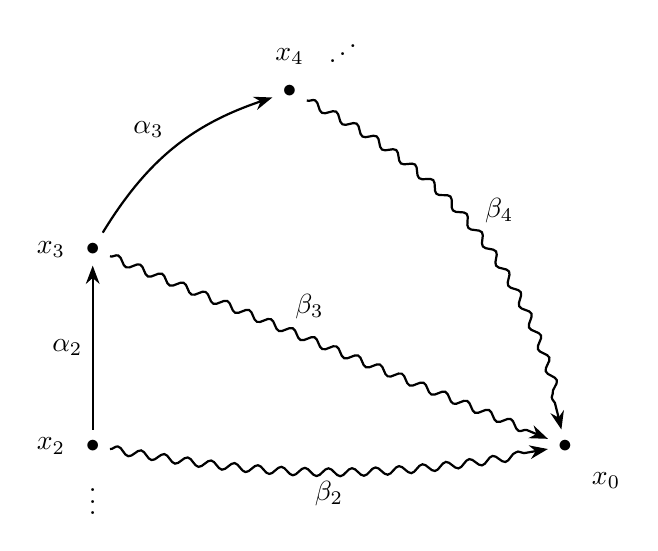
\begin{tikzpicture}[
            >=Stealth, 
            auto, 
            node distance=2cm, 
            thick,
            slinky arrow/.style={
                ->,
                decorate,
                decoration={snake, amplitude=0.5mm, segment length=3mm, post length=2mm}
            }
        ]
            \node[label=left:$x_2$] (x2) at (0,0) {$\bullet$};
            \node[label=left:$x_3$] (x3) at (0,2.5) {$\bullet$};
            \node[label=above:$x_4$] (x4) at (2.5,4.5) {$\bullet$};
            \node[label=below right:$x_0$] (x0) at (6,0) {$\bullet$};
            \node at (0, -0.6) {$\vdots$}; 
            \node[rotate=35] at (3.2, 5) {$\dots$}; 
            \draw[->] (x2) -- node[left] {$\alpha_2$} (x3);
            \draw[->] (x3) to[bend left=20] node[above left] {$\alpha_3$} (x4);
            
            \draw[slinky arrow] (x2) to[bend right=10] node[below] {$\beta_2$} (x0);
            \draw[slinky arrow] (x3) -- node[pos=0.4, above right] {$\beta_3$} (x0); 
            \draw[slinky arrow] (x4) to[bend left=25] node[above right] {$\beta_4$} (x0);
        \end{tikzpicture}
    \end{center}
    These are closed paths at \(x_0\) with
    \[\alpha \simeq \gamma_1 * \gamma_2 * \cdots * \gamma_n\]
\end{snippetproof}

\begin{snippetcorollary}{simply-connected-union}{Simply connected union}
    Let \(X = A \union B\) where \(A, B, A \intersection B\) are
    arc-connected open subsets.
    If \(A\), \(B\), and \(A \intersection B\) are all simply connected,
    then \(X\) is simply connected.
\end{snippetcorollary}

\begin{snippetproof}{simply-connected-union-proof}{simply-connected-union}{Simply connected union}
    \(X\) is arc-connected as a union of two arc-connected subsets with non-empty intersection.
    Since \(\pi_1(A, x_0)\) and \(\pi_1(B, x_0)\) are trivial,
    and \(\pi_1(X, x_0)\) is generated by their images, it is also trivial.
\end{snippetproof}

\begin{snippettheorem}{sphere-simply-connected}{Spheres are simply connected}
    For \(n \geq 2\), the sphere \(S^n\) is simply connected,
    i.e., \(\pi_1(S^n) = \{e\}\).
\end{snippettheorem}

\begin{snippetproof}{sphere-simply-connected-proof}{sphere-simply-connected}{Spheres are simply connected}
    Write \(S^n = A \union B\) where
    \(A = S^n \difference \{N\}\) (removing north pole) and
    \(B = S^n \difference \{S\}\) (removing south pole).
    
    Both \(A\) and \(B\) are homeomorphic to \(\realnumbers^n\),
    hence contractible and simply connected.
    
    The intersection \(A \intersection B = S^n \difference \{N, S\}\)
    is homeomorphic to \(\realnumbers^n \difference \{0\}\),
    which for \(n \geq 2\) is arc-connected.
    Moreover, \(S^{n-1}\) is a deformation retract of \(\realnumbers^n \difference \{0\}\).
    
    For \(n \geq 2\), this intersection is arc-connected and,
    applying inductively (or noting that \(S^1\) paths can be deformed),
    the result follows from Van Kampen.
\end{snippetproof}

\end{document}
